% Created by tikzDevice version 0.12.3.1 on 2021-06-11 18:34:39
% !TEX encoding = UTF-8 Unicode
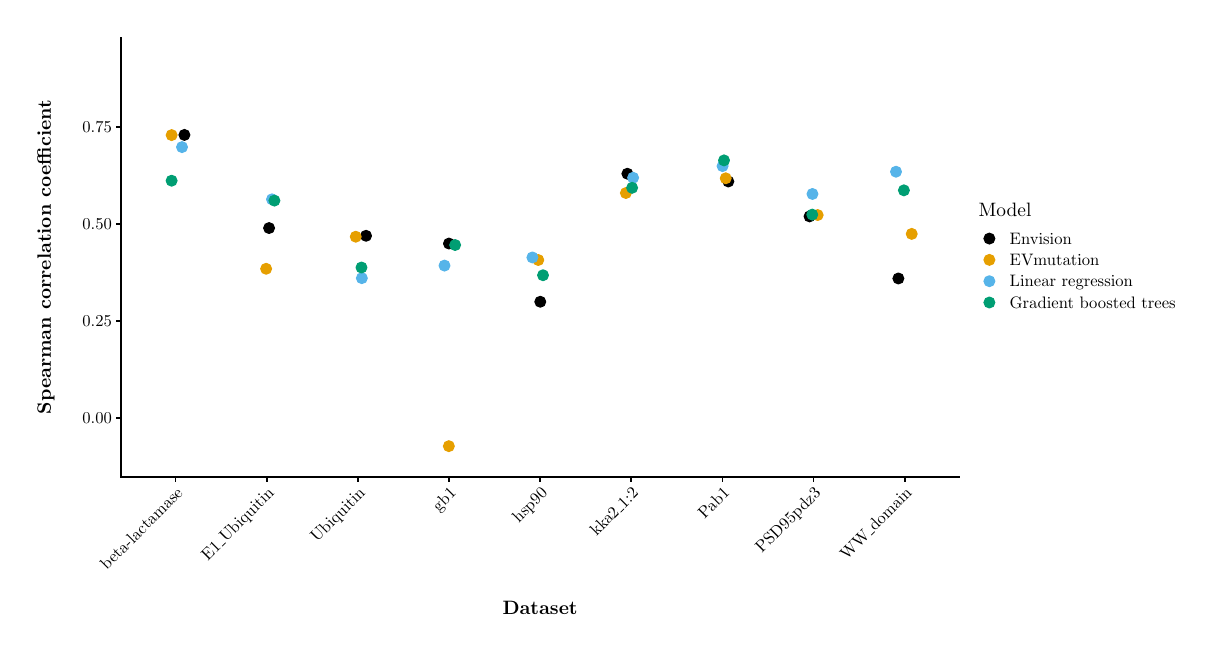
\begin{tikzpicture}[x=1pt,y=1pt]
	\definecolor{fillColor}{RGB}{255,255,255}
	\path[use as bounding box,fill=fillColor,fill opacity=0.00] (0,0) rectangle (418.34,216.81);
	\begin{scope}
		\path[clip] ( 33.67, 54.47) rectangle (336.66,213.31);
		\definecolor{drawColor}{RGB}{0,0,0}
		\definecolor{fillColor}{RGB}{0,0,0}

		\path[draw=drawColor,line width= 0.4pt,line join=round,line cap=round,fill=fillColor] ( 56.64,178.05) circle (  1.96);

		\path[draw=drawColor,line width= 0.4pt,line join=round,line cap=round,fill=fillColor] (253.18,161.23) circle (  1.96);

		\path[draw=drawColor,line width= 0.4pt,line join=round,line cap=round,fill=fillColor] ( 87.23,144.40) circle (  1.96);

		\path[draw=drawColor,line width= 0.4pt,line join=round,line cap=round,fill=fillColor] (216.71,164.03) circle (  1.96);

		\path[draw=drawColor,line width= 0.4pt,line join=round,line cap=round,fill=fillColor] (282.52,148.61) circle (  1.96);

		\path[draw=drawColor,line width= 0.4pt,line join=round,line cap=round,fill=fillColor] (314.63,126.18) circle (  1.96);

		\path[draw=drawColor,line width= 0.4pt,line join=round,line cap=round,fill=fillColor] (122.27,141.60) circle (  1.96);

		\path[draw=drawColor,line width= 0.4pt,line join=round,line cap=round,fill=fillColor] (152.23,138.80) circle (  1.96);

		\path[draw=drawColor,line width= 0.4pt,line join=round,line cap=round,fill=fillColor] (185.23,117.77) circle (  1.96);
		\definecolor{drawColor}{RGB}{230,159,0}
		\definecolor{fillColor}{RGB}{230,159,0}

		\path[draw=drawColor,line width= 0.4pt,line join=round,line cap=round,fill=fillColor] ( 52.02,177.99) circle (  1.96);

		\path[draw=drawColor,line width= 0.4pt,line join=round,line cap=round,fill=fillColor] ( 86.17,129.68) circle (  1.96);

		\path[draw=drawColor,line width= 0.4pt,line join=round,line cap=round,fill=fillColor] (118.55,141.27) circle (  1.96);

		\path[draw=drawColor,line width= 0.4pt,line join=round,line cap=round,fill=fillColor] (152.19, 65.59) circle (  1.96);

		\path[draw=drawColor,line width= 0.4pt,line join=round,line cap=round,fill=fillColor] (184.51,132.85) circle (  1.96);

		\path[draw=drawColor,line width= 0.4pt,line join=round,line cap=round,fill=fillColor] (216.16,157.06) circle (  1.96);

		\path[draw=drawColor,line width= 0.4pt,line join=round,line cap=round,fill=fillColor] (252.24,162.38) circle (  1.96);

		\path[draw=drawColor,line width= 0.4pt,line join=round,line cap=round,fill=fillColor] (285.46,149.10) circle (  1.96);

		\path[draw=drawColor,line width= 0.4pt,line join=round,line cap=round,fill=fillColor] (319.45,142.29) circle (  1.96);
		\definecolor{drawColor}{RGB}{86,180,233}
		\definecolor{fillColor}{RGB}{86,180,233}

		\path[draw=drawColor,line width= 0.4pt,line join=round,line cap=round,fill=fillColor] (218.77,162.58) circle (  1.96);

		\path[draw=drawColor,line width= 0.4pt,line join=round,line cap=round,fill=fillColor] (182.38,133.78) circle (  1.96);

		\path[draw=drawColor,line width= 0.4pt,line join=round,line cap=round,fill=fillColor] (251.10,166.79) circle (  1.96);

		\path[draw=drawColor,line width= 0.4pt,line join=round,line cap=round,fill=fillColor] (150.62,130.84) circle (  1.96);

		\path[draw=drawColor,line width= 0.4pt,line join=round,line cap=round,fill=fillColor] (120.75,126.30) circle (  1.96);

		\path[draw=drawColor,line width= 0.4pt,line join=round,line cap=round,fill=fillColor] ( 88.28,154.78) circle (  1.96);

		\path[draw=drawColor,line width= 0.4pt,line join=round,line cap=round,fill=fillColor] (283.58,156.72) circle (  1.96);

		\path[draw=drawColor,line width= 0.4pt,line join=round,line cap=round,fill=fillColor] (313.77,164.76) circle (  1.96);

		\path[draw=drawColor,line width= 0.4pt,line join=round,line cap=round,fill=fillColor] ( 55.77,173.65) circle (  1.96);
		\definecolor{drawColor}{RGB}{0,158,115}
		\definecolor{fillColor}{RGB}{0,158,115}

		\path[draw=drawColor,line width= 0.4pt,line join=round,line cap=round,fill=fillColor] (218.41,158.94) circle (  1.96);

		\path[draw=drawColor,line width= 0.4pt,line join=round,line cap=round,fill=fillColor] (186.22,127.35) circle (  1.96);

		\path[draw=drawColor,line width= 0.4pt,line join=round,line cap=round,fill=fillColor] (251.62,168.85) circle (  1.96);

		\path[draw=drawColor,line width= 0.4pt,line join=round,line cap=round,fill=fillColor] (154.46,138.27) circle (  1.96);

		\path[draw=drawColor,line width= 0.4pt,line join=round,line cap=round,fill=fillColor] (120.62,130.14) circle (  1.96);

		\path[draw=drawColor,line width= 0.4pt,line join=round,line cap=round,fill=fillColor] ( 89.16,154.32) circle (  1.96);

		\path[draw=drawColor,line width= 0.4pt,line join=round,line cap=round,fill=fillColor] (283.51,149.26) circle (  1.96);

		\path[draw=drawColor,line width= 0.4pt,line join=round,line cap=round,fill=fillColor] (316.62,158.03) circle (  1.96);

		\path[draw=drawColor,line width= 0.4pt,line join=round,line cap=round,fill=fillColor] ( 52.01,161.51) circle (  1.96);
	\end{scope}
	\begin{scope}
		\path[clip] (  0.00,  0.00) rectangle (418.34,216.81);
		\definecolor{drawColor}{RGB}{0,0,0}

		\path[draw=drawColor,line width= 0.6pt,line join=round,line cap=rect] ( 33.67, 54.47) --
		( 33.67,213.31);
	\end{scope}
	\begin{scope}
		\path[clip] (  0.00,  0.00) rectangle (418.34,216.81);
		\definecolor{drawColor}{RGB}{0,0,0}

		\node[text=drawColor,anchor=base east,inner sep=0pt, outer sep=0pt, scale=  0.60] at ( 30.42, 73.64) {0.00};

		\node[text=drawColor,anchor=base east,inner sep=0pt, outer sep=0pt, scale=  0.60] at ( 30.42,108.69) {0.25};

		\node[text=drawColor,anchor=base east,inner sep=0pt, outer sep=0pt, scale=  0.60] at ( 30.42,143.74) {0.50};

		\node[text=drawColor,anchor=base east,inner sep=0pt, outer sep=0pt, scale=  0.60] at ( 30.42,178.79) {0.75};
	\end{scope}
	\begin{scope}
		\path[clip] (  0.00,  0.00) rectangle (418.34,216.81);
		\definecolor{drawColor}{RGB}{0,0,0}

		\path[draw=drawColor,line width= 0.6pt,line join=round] ( 31.92, 75.71) --
		( 33.67, 75.71);

		\path[draw=drawColor,line width= 0.6pt,line join=round] ( 31.92,110.76) --
		( 33.67,110.76);

		\path[draw=drawColor,line width= 0.6pt,line join=round] ( 31.92,145.81) --
		( 33.67,145.81);

		\path[draw=drawColor,line width= 0.6pt,line join=round] ( 31.92,180.86) --
		( 33.67,180.86);
	\end{scope}
	\begin{scope}
		\path[clip] (  0.00,  0.00) rectangle (418.34,216.81);
		\definecolor{drawColor}{RGB}{0,0,0}

		\path[draw=drawColor,line width= 0.6pt,line join=round,line cap=rect] ( 33.67, 54.47) --
		(336.66, 54.47);
	\end{scope}
	\begin{scope}
		\path[clip] (  0.00,  0.00) rectangle (418.34,216.81);
		\definecolor{drawColor}{RGB}{0,0,0}

		\path[draw=drawColor,line width= 0.6pt,line join=round] ( 53.43, 52.72) --
		( 53.43, 54.47);

		\path[draw=drawColor,line width= 0.6pt,line join=round] ( 86.36, 52.72) --
		( 86.36, 54.47);

		\path[draw=drawColor,line width= 0.6pt,line join=round] (119.30, 52.72) --
		(119.30, 54.47);

		\path[draw=drawColor,line width= 0.6pt,line join=round] (152.23, 52.72) --
		(152.23, 54.47);

		\path[draw=drawColor,line width= 0.6pt,line join=round] (185.17, 52.72) --
		(185.17, 54.47);

		\path[draw=drawColor,line width= 0.6pt,line join=round] (218.10, 52.72) --
		(218.10, 54.47);

		\path[draw=drawColor,line width= 0.6pt,line join=round] (251.03, 52.72) --
		(251.03, 54.47);

		\path[draw=drawColor,line width= 0.6pt,line join=round] (283.97, 52.72) --
		(283.97, 54.47);

		\path[draw=drawColor,line width= 0.6pt,line join=round] (316.90, 52.72) --
		(316.90, 54.47);
	\end{scope}
	\begin{scope}
		\path[clip] (  0.00,  0.00) rectangle (418.34,216.81);
		\definecolor{drawColor}{RGB}{0,0,0}

		\node[text=drawColor,rotate= 45.00,anchor=base east,inner sep=0pt, outer sep=0pt, scale=  0.60] at ( 56.35, 48.30) {beta-lactamase};

		\node[text=drawColor,rotate= 45.00,anchor=base east,inner sep=0pt, outer sep=0pt, scale=  0.60] at ( 89.29, 48.30) {E1\_Ubiquitin};

		\node[text=drawColor,rotate= 45.00,anchor=base east,inner sep=0pt, outer sep=0pt, scale=  0.60] at (122.22, 48.30) {Ubiquitin};

		\node[text=drawColor,rotate= 45.00,anchor=base east,inner sep=0pt, outer sep=0pt, scale=  0.60] at (155.15, 48.30) {gb1};

		\node[text=drawColor,rotate= 45.00,anchor=base east,inner sep=0pt, outer sep=0pt, scale=  0.60] at (188.09, 48.30) {hsp90};

		\node[text=drawColor,rotate= 45.00,anchor=base east,inner sep=0pt, outer sep=0pt, scale=  0.60] at (221.02, 48.30) {kka2\_1:2};

		\node[text=drawColor,rotate= 45.00,anchor=base east,inner sep=0pt, outer sep=0pt, scale=  0.60] at (253.96, 48.30) {Pab1};

		\node[text=drawColor,rotate= 45.00,anchor=base east,inner sep=0pt, outer sep=0pt, scale=  0.60] at (286.89, 48.30) {PSD95pdz3};

		\node[text=drawColor,rotate= 45.00,anchor=base east,inner sep=0pt, outer sep=0pt, scale=  0.60] at (319.82, 48.30) {WW\_domain};
	\end{scope}
	\begin{scope}
		\path[clip] (  0.00,  0.00) rectangle (418.34,216.81);
		\definecolor{drawColor}{RGB}{0,0,0}

		\node[text=drawColor,anchor=base,inner sep=0pt, outer sep=0pt, scale=  0.70] at (185.17,  4.86) {\bfseries Dataset};
	\end{scope}
	\begin{scope}
		\path[clip] (  0.00,  0.00) rectangle (418.34,216.81);
		\definecolor{drawColor}{RGB}{0,0,0}

		\node[text=drawColor,rotate= 90.00,anchor=base,inner sep=0pt, outer sep=0pt, scale=  0.70] at (  8.39,133.89) {\bfseries Spearman correlation coefficient};
	\end{scope}
	\begin{scope}
		\path[clip] (  0.00,  0.00) rectangle (418.34,216.81);
		\definecolor{drawColor}{RGB}{0,0,0}

		\node[text=drawColor,anchor=base west,inner sep=0pt, outer sep=0pt, scale=  0.70] at (343.66,148.63) {Model};
	\end{scope}
	\begin{scope}
		\path[clip] (  0.00,  0.00) rectangle (418.34,216.81);
		\definecolor{drawColor}{RGB}{0,0,0}
		\definecolor{fillColor}{RGB}{0,0,0}

		\path[draw=drawColor,line width= 0.4pt,line join=round,line cap=round,fill=fillColor] (347.51,140.60) circle (  1.96);
	\end{scope}
	\begin{scope}
		\path[clip] (  0.00,  0.00) rectangle (418.34,216.81);
		\definecolor{drawColor}{RGB}{230,159,0}
		\definecolor{fillColor}{RGB}{230,159,0}

		\path[draw=drawColor,line width= 0.4pt,line join=round,line cap=round,fill=fillColor] (347.51,132.90) circle (  1.96);
	\end{scope}
	\begin{scope}
		\path[clip] (  0.00,  0.00) rectangle (418.34,216.81);
		\definecolor{drawColor}{RGB}{86,180,233}
		\definecolor{fillColor}{RGB}{86,180,233}

		\path[draw=drawColor,line width= 0.4pt,line join=round,line cap=round,fill=fillColor] (347.51,125.20) circle (  1.96);
	\end{scope}
	\begin{scope}
		\path[clip] (  0.00,  0.00) rectangle (418.34,216.81);
		\definecolor{drawColor}{RGB}{0,158,115}
		\definecolor{fillColor}{RGB}{0,158,115}

		\path[draw=drawColor,line width= 0.4pt,line join=round,line cap=round,fill=fillColor] (347.51,117.50) circle (  1.96);
	\end{scope}
	\begin{scope}
		\path[clip] (  0.00,  0.00) rectangle (418.34,216.81);
		\definecolor{drawColor}{RGB}{0,0,0}

		\node[text=drawColor,anchor=base west,inner sep=0pt, outer sep=0pt, scale=  0.60] at (354.86,138.53) {Envision};
	\end{scope}
	\begin{scope}
		\path[clip] (  0.00,  0.00) rectangle (418.34,216.81);
		\definecolor{drawColor}{RGB}{0,0,0}

		\node[text=drawColor,anchor=base west,inner sep=0pt, outer sep=0pt, scale=  0.60] at (354.86,130.83) {EVmutation};
	\end{scope}
	\begin{scope}
		\path[clip] (  0.00,  0.00) rectangle (418.34,216.81);
		\definecolor{drawColor}{RGB}{0,0,0}

		\node[text=drawColor,anchor=base west,inner sep=0pt, outer sep=0pt, scale=  0.60] at (354.86,123.13) {Linear regression};
	\end{scope}
	\begin{scope}
		\path[clip] (  0.00,  0.00) rectangle (418.34,216.81);
		\definecolor{drawColor}{RGB}{0,0,0}

		\node[text=drawColor,anchor=base west,inner sep=0pt, outer sep=0pt, scale=  0.60] at (354.86,115.43) {Gradient boosted trees};
	\end{scope}
\end{tikzpicture}%
